\documentclass[border=2pt]{standalone}
% Shared TikZ styles for the memory-architecture diagrams (compiled as standalone PDFs).
\usepackage[T1]{fontenc}
\usepackage{lmodern}
\usepackage[english]{babel}
\usepackage{tikz}
\usetikzlibrary{positioning,fit,arrows.meta,calc,backgrounds,shapes.geometric}
\definecolor{procFill}{HTML}{E8F1FB}\definecolor{procLine}{HTML}{2A78D6}
\definecolor{memFill}{HTML}{EAF7F1}\definecolor{memLine}{HTML}{1BAF7A}
\definecolor{wFill}{HTML}{FFF6E0}\definecolor{wLine}{HTML}{EDA100}
\definecolor{slowRed}{HTML}{E34948}\definecolor{boxLine}{HTML}{9A9890}\definecolor{ink2}{HTML}{52514E}
\tikzset{
  every node/.style={font=\small, align=center},
  proc/.style={rectangle, rounded corners=2pt, draw=procLine, fill=procFill, very thick, minimum height=2.4em, inner sep=3pt},
  mem/.style={rectangle, draw=memLine, fill=memFill, very thick, inner sep=4pt},
  weights/.style={rectangle, draw=wLine, fill=wFill, thick, font=\footnotesize, inner sep=2pt},
  box/.style={draw=boxLine, dashed, rounded corners=3pt, inner sep=6pt},
  boxlabel/.style={font=\footnotesize\bfseries, text=ink2},
  bus/.style={line width=#1, ink2},
  buslabel/.style={font=\footnotesize, text=ink2, fill=white, inner sep=1pt},
}

\begin{document}
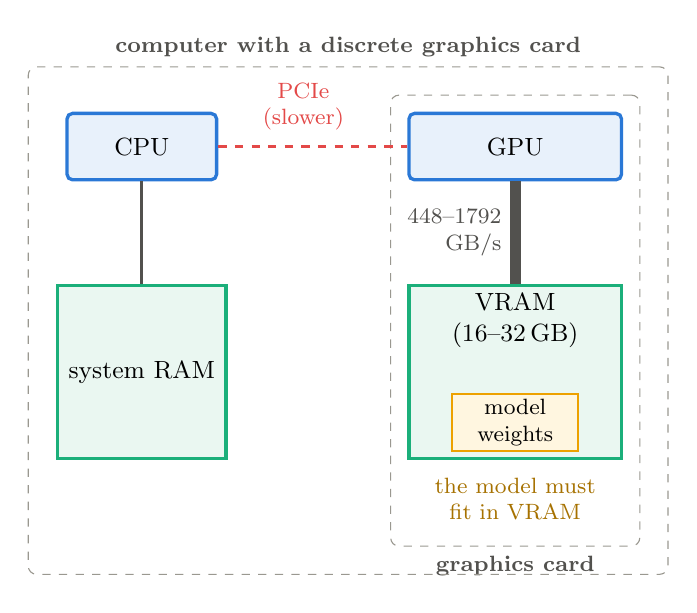
\begin{tikzpicture}
  \node[proc, minimum width=1.9cm] (cpu) {CPU};
  \node[mem, minimum width=1.9cm, minimum height=2.2cm, below=13mm of cpu] (ram) {system RAM};
  \node[proc, minimum width=2.7cm, right=24mm of cpu] (gpu) {GPU};
  \node[mem, minimum width=2.7cm, minimum height=2.2cm, below=13mm of gpu, align=center] (vram) {};
  \node[font=\small, anchor=north] at (vram.north) {VRAM\\(16--32\,GB)};
  \node[weights, minimum width=1.6cm, anchor=south] at ([yshift=3pt]vram.south) {model\\weights};
  \node[font=\footnotesize, text=wLine!70!black, below=1mm of vram] (vnote) {the model must\\fit in VRAM};
  \draw[bus=1.2pt] (cpu) -- (ram);
  \draw[bus=4pt] (gpu) -- node[buslabel, left=2pt, align=right] {448--1792\\GB/s} (vram);
  \draw[slowRed, line width=1.2pt, dashed] (cpu) -- node[above=2pt, pos=0.45, font=\footnotesize, text=slowRed, align=center] {PCIe\\(slower)} (gpu);
  \begin{scope}[on background layer]
    \node[box, fit=(gpu)(vram)(vnote), label={[boxlabel]below:graphics card}] (card) {};
    \node[box, inner sep=10pt, fit=(cpu)(ram)(card)(card.south), label={[boxlabel]above:computer with a discrete graphics card}] {};
  \end{scope}
  \end{tikzpicture}
\end{document}
